% !TEX root = ../main.tex
\chapter{DNA分子的释放过程简述}

\section{DNA/$\ce{Zr^{4+}}$层层自组装结构}
\subsection{组装过程}
多层膜的制造过程包括
三步:清洗金薄膜,孵化金
薄膜和$\ce{Zr^{4+}}$/ssDNA的循环沉积
直到达到所需的层数为止,如图~\ref{fig:incubation_process}所示。

1)清洗金薄膜:使用去离子水对金薄膜进行除尘,
然后将金薄膜放入丙酮($\ce{C3H6O}$)中煮沸10分钟,
再次用去离子水清洗。再将金薄膜放入无水乙醇中煮沸10分钟,
再次用去离子水清洗。

2)孵化金薄膜:将清洗后的金薄膜MUA(巯基十一酸)溶液溶液中浸泡一晚后,
再次使用去离子水清洗。

3)$\ce{Zr^{4+}}$/ssDNA的循环沉积:将金薄膜浸入$0.1mM$的$\ce{Zr^{4+}}$溶液5分钟,
再浸入$0.1mg/mL$的ssDNA溶液5分钟,接着使用纯化水冲洗,即可得到$\ce{Zr^{4+}}$/ssDNA
双层结构,重复这一过程至所需的层数。最后,使用氮气对组装好的多层膜进行干燥。

\begin{figure}[H]
    \centering
    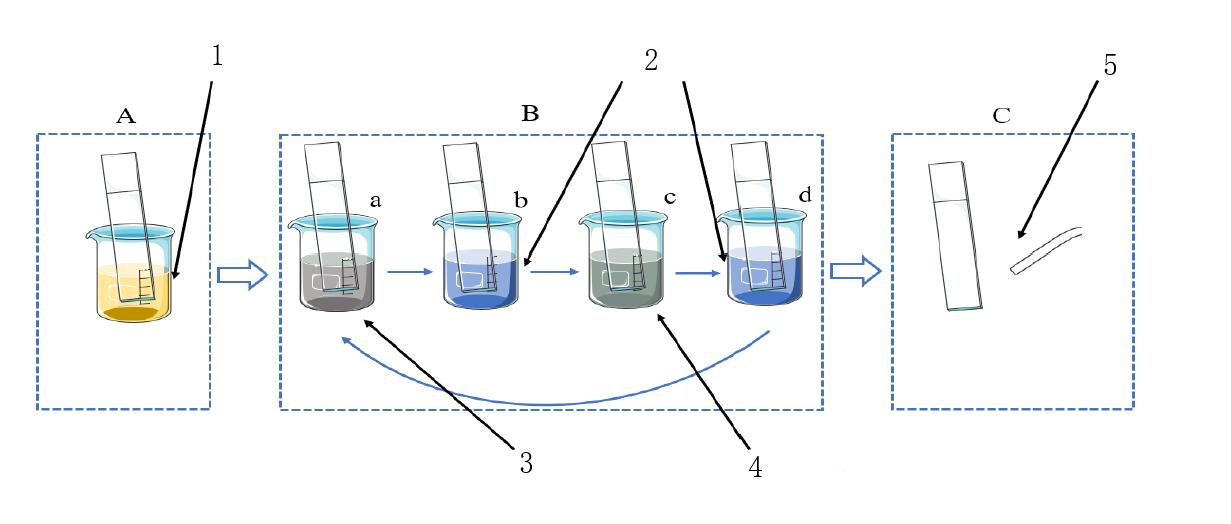
\includegraphics[scale=0.5]{Incubation process and repeated cyclic deposition process.jpg}\\
    1)MUA乙醇溶液 2)纯化水 3)$\ce{Zr^{4+}}$溶液 \\
    4)ssDNA溶液 5)氮气\\
    \caption{DNA/$\ce{Zr^{4+}}$层层自组装结构组装过程}
    \label{fig:incubation_process}
\end{figure}

\subsection{理化性质}
根据扫描隧道显微镜(STM)的扫描结果,组装成的多次膜结构中,$\ce{Zr^{4+}}$在
平面上均匀分布,根据信号峰值的间距可以得到$\ce{Zr^{4+}}$之间的距离为3~4$nm$
,$\ce{Zr^{4+}}$/ssDNA的厚度约为5$nm$\cite{Shervedani2011Electrochemical}。

电化学特性方面,根据实验测定\cite{Karimi2011}多层膜结构组成的电极的电荷转移电阻为$136.5\pm1.8k\Omega$,
双电层电容为$1.89\pm0.06\mu F$,赝电容为$0.46\pm0.04\mu F$。


\section{层层自组装结构受控分解的原理}
\subsection{电信号激励下的电化学反应}
标准电极电位的大小反映了电极在进行电极反应时,相对于标准氢电极的得失电子的能力。
标准电极电位的值越大,就越容易获得电子,换句话说它的氧化性就越强;反之,
标准电极电位的值越小,就越容易失去电子,换句话说它的还原就越强\cite{Trasatti1980}。
将常见的物质的标准电极电位排列得到一个序列,称为电化学序(Electrochemical Series)。

由于溶液环境中,主要成分是氯化钠($\ce{NaCl}$)。根据溶液里潜在反应物质的电化学序提供的信息\cite{Weik2001}
\footnote{在实验用溶液中初始$\ce{pH=7}$,即在溶液中$c_{\ce{OH-}}=c_{\ce{H+}}=10^{-7}mM$
这时由于$\ce{OH-}$与$\ce{H+}$的浓度处于一个极低的水平,我们认为是$\ce{H2O}$参与了反应,
所以采用了$\ce{H2O}$的标准电极电位。}:
\begin{align}
\label{equation:anode_reaction} \ce{Cl2(g) + 2e- &<=> 2 Cl-} \quad\quad\quad\quad &{E°}=1.35827V \\
\ce{O2(g) + 4H+ + 4 e- &<=> 2H2O} &{E°}=1.229V \\ 
\label{equation:cathode_reaction} \ce{2 H2O + 2 e- &<=> H2(g) + 2OH- } &{E°}=-0.8277V \\
\ce{Zr^4+ + 4e- &<=> Zr}   &{E°}=-1.45V \\
\ce{Na+ + e- &<=> Na }     &{E°}=-2.71V
\end{align}


在施加电信号的时,阴极处,$\ce{H2O}$分子的氧化性强于$\ce{Zr^4+}$离子与$\ce{Na+}$离子
($E°=–0.8277V>-1.45V>–2.71V$),所以释放的电子会优先被$\ce{H2O}$分子获取,反应生成
$\ce{H2}$气体与$\ce{OH-}$离子;阳极处,$\ce{Cl-}$离子的还原性强于$\ce{H2O}$分子
($E°=-1.35827V<-1.229V$),所以$\ce{Cl-}$离子会优先释放电子,反应生成$\ce{Cl2}$气体。

\subsection{Zr$^{4+}$水解过程}
考虑如下的反应式:
\begin{equation}
    \ce{\alpha{A} +\beta{B} <=> \rho{R} + \sigma{S}}
\end{equation}

对某一可逆反应,在一定温度下,反应达到平衡状态后,反应物与生成物热力学活性的系数次方的比是一个常数,
称为化学反应的平衡常数$K°$(equilibrium constant):
\begin{equation}
    K°=\frac{\{R\}^\rho \{S\}^\sigma}{\{A\}^\alpha \{B\}^\beta}
\end{equation}

其中,{$\{X\}$}表示的是物质$X$在平衡状态下的热力学活性,基于底物的浓度。
研究者们发现实际反应与理论值存在有偏差的情况,这时我们使用活性系数修正底物的浓度,
以弥补偏离理想的情况\cite{Königsberger2017}。
在本文所涉及的反应中,均可以将热力学活性数值上等同于浓度。平衡常数越大,则正向反应越彻底。

对于水,会有如下可逆反应:
\begin{equation}
    \ce{H2O <=> H+ + OH-} \quad K°=K_w
\end{equation}

我们称之为水的电离反应,其中$K_w$被称为水的离子积,随温度变化而变化,在$25°C$时,$k_w=10^{-14}$。
它表明了在水溶液中,温度一定的情况下,溶液环境里的$c_{\ce{OH-}}$与$c_{\ce{H+}}$的乘积是一个定值。

如反应式 ~\ref{equation:cathode_reaction} 所示,随着电化学反应的进行,在阴极区域会不断产生$\ce{OH-}$
离子,从而抑制水的电离,降低了$c_{\ce{H+}}$。

考虑$\ce{Zr^4+}$的水解反应\cite{Thoenen2004Development}:
\begin{equation}
    \ce{Zr^4+ +2 H2O  = ZrO2 + 4H+} \quad lgK°=1.9
    \label{Zr4+水解}
\end{equation}

$c_{\ce{H+}}$的降低会促进水解反应的发生,这会导致固定在LBL结构中的$\ce{Zr^4+}$不断水解成$\ce{ZrO2}$,
从而引起LBL结构的分解,并释放出DNA分子。

\subsection{电场影响下DNA分子运动}
DNA分子的骨架由大量的磷酸基团脱水缩合连接,磷酸骨架的每个残基带有一个负电荷,所以DNA分子整体是带负电荷的
\cite{Lipfert2014}。在电信号的激励下,DNA会向远离极板的方向移动;而$\ce{Zr^4+}$带正电荷,会向靠近极板的方向
移动,并阻碍DNA分子的扩散。所以只有在$\ce{Zr^4+}$被水解反应消耗后,DNA才会被释放。

\subsection{反应过程总述}
在电信号的激励下,阴极处会发生式~\ref{equation:cathode_reaction}
所描述的化学反应,这使得阴极处$\ce{OH-}$浓度增加,促使$\ce{Zr^4+}$
发生式~\ref{Zr4+水解}描述的水解反应,$\ce{Zr^4+}$的消耗导致了
DNA/$\ce{Zr^{4+}}$层层自组装结构的分解,被释放到溶液中的DNA在
浓度梯度力与电场力的共同作用下,在溶液中扩散。
%缺图

\section{基本控制方程}
\subsection{扩散定律}
菲克定律由阿道夫·菲克于十九世纪提出,对扩散给出了最简单的描述:
\begin{itemize}[leftmargin=40pt]
    \item [1)]由扩散引起的摩尔通量与浓度梯度成正比。
    \item [2)]空间上某一点的浓度变化率与浓度的空间二阶导数成正比。
\end{itemize}

菲克第一定律可以表示为:
\begin{equation}
    \mathbf{N_i}=-D_i\nabla{c_i}
\end{equation}

对于物质$i$,$\mathbf{N_i}$是摩尔通量($mol\cdot{m^{-2}\cdot{s^{-1}}}$),$D_i$是扩散系数($m^2\cdot{s^{-1}}$),$c_i$是浓度($mol\cdot{m^{-3}}$)。
根据连续性方程:
\begin{equation}
    \frac{\partial c_i}{\partial t}+\nabla\cdot{N_i}=0
    \label{eqation:continuity}
\end{equation}

可以推导出菲克第二定律:
\begin{equation}
    \frac{\partial c_i}{\partial t}=D_i\nabla^2{c_i}
    \label{fick's 2nd}
\end{equation}

在稀溶液中,我们假设$D_i$是一个常数。它描述了自由扩散时,浓度随时间的变化关系\cite{Sakaguchi2018} 。
\subsection{Nernst-Einstein 关系}
考虑外力作用于扩散粒子:
\begin{equation}
    \mathbf{v_d}=m_{abs}\mathbf{F}
\end{equation}

在这一本构关系中,$\mathbf{v_d}$表示漂移速度($m\cdot{s^{-1}}$),
$m_{abs}$是绝对迁移率($N\cdot{s\cdot{m^{-1}}}$),$F$是作用力($N$)。
考虑浓度梯度力同时作用于粒子,粒子的总通量$\mathbf{N_i}$可以表达为:
\begin{equation}
    \mathbf{N_i}=-D_i\nabla{c_i}+m_{i,abs}c_i\mathbf{F}
\end{equation}

当总通量为$0$时,扩散作用于迁移作用引起的通量大小相等且方向相反:
\begin{equation}
    \nabla{c_i}=\frac{m_{i,abs}}{D_i}c_i\mathbf{F}
\end{equation}

各个方向上的净通量为$0$时,可以假设扩散与迁移达到平衡。此时的浓度分部可以用Boltzmann方程来描述:
\begin{equation}
    c_i=c_{i,0}exp(-\frac{U}{kT})
\end{equation}

其中,$c_{i,0}$表示势能为零时的浓度($mol\cdot{m^{-3}}$),$U$表示分子的势能($J$),
$k$表示Boltzmann常数($J\cdot{K^{-1}}$),T是绝对温度(K)。此时该浓度场的梯度为:
\begin{equation}
    \nabla{c_i}=-c_{i,0}exp(-\frac{U}{kT})\frac{1}{kT}\nabla{U}
\end{equation}

根据定义,力是势能的负梯度:
\begin{equation}
    \mathbf{F}=-\nabla{U}
\end{equation}

结合等式(2-7)与(2-9):
\begin{equation}
    \frac{m_{i,abs}}{D_i}c_i\mathbf{F}=\frac{1}{kT}c_i\mathbf{F}
\end{equation}

化简后得到:
\begin{equation}
    m_{i,abs}=\frac{D_i}{kT}
    \label{Nernst-Einstein}
\end{equation}

该等式描述了带点粒子的扩散系数$D_i$与扩散迁移率$m_{i,abs}$的关系,被称为Nernst-Einstein关系\cite{Mehrer2007,CONWAY1972250}。
\subsection{Nernst-Planck 方程}
在电场作用下,带电粒子受到电场力$\mathbf{F}$:
\begin{equation}
    \mathbf{F}=-z_ie_0\nabla\phi
\end{equation}

其中,$z_i$表示粒子的电荷数,$e_0$是电子的基本电荷,$\phi$是电势($V$),$−\nabla{\phi}$ 表示电场。
我们定义$u_i=e_0m_{abs}$为该粒子的电化学迁移率,此时,漂移速度可由下式求得:
\begin{equation}
   \mathbf{v_d}=-z_iu_i\nabla\phi
\end{equation}

由此得到的离子$i$的迁移通量是漂移速度$v_d$和离子浓度$c_i$的乘积,此通量的贡献称为离子迁移或电迁移:
\begin{equation}
    \mathbf{N_{i,migr}}=-z_iu_ic_i\nabla\phi
\end{equation}

在一般的稀释电解质中,通量贡献可能有以下三种来源:扩散、迁移和对流:
\begin{equation}
    N_i=-\overbrace{D_i\nabla{c_i}}^{Diff}-\overbrace{z_iu_ic_i\nabla\phi}^{Migr}+\overbrace{c_i\mathbf{u}}^{Conv}
\end{equation}

其中$\mathbf{u}$是电解质速度($m\cdot{s^{-1}}$)。由Nernst-Einstein关系我们得到电化学迁移率$u_i$与扩散率$D_i$的关系。
代入到式(2-2)的连续性方程:
\begin{equation}
    \frac{\partial c_i}{\partial t}=\nabla{(D_i\nabla{c_i}+\frac{D_iz_ie_0}{kT}c_i\nabla\phi+c_i\mathbf{u})}
    \label{equation:Nernst_Planck}
\end{equation}

该等式描述了流体介质中带电化学物质的运动情况,被称为Nernst–Planck方程\cite{Mehrer2007}。
\subsection{离子迁移}
电解质中的电流密度$\mathbf{i}$可以通过该电解质中所有离子的贡献之和求得:
\begin{equation}
    \mathbf{i}=F\sum_i{z_i\mathbf{N_i}}
\end{equation}

式中,$F$为法拉第常数。将式(2-15)的通量代入到该方程,可以得到:
\begin{equation}
    \mathbf{i}=F\sum_i(-z_iD_i\nabla{c_i}-z_i^2u_ic_i\nabla\phi)+F\sum_iz_ic_i
\end{equation}

在大多数电化学反应中,除双电层区域外,都可以假设电解质呈电中性:
\begin{equation}
    F\sum_iz_ic_i=0
    \label{equation:neutrality}
\end{equation}

对流使得浓度保持均匀的分布,因此,在靠近电极的区域外,电解槽中的任何位置都具有恒定的电导率$\kappa$,电流密度表达式变为:
\begin{equation}
    \mathbf{i}=-\overbrace{F\sum_i(z_i^2u_ic_i)}^{Conductivity,\kappa}\nabla\phi
\end{equation}

这个方程表明,组成恒定的电解质中的电流完全由迁移产生。电流遵循欧姆定律,电导率由电解质中每个组成离子的迁移贡献总和决定\cite{Smedley1980}。

\subsection{化学反应速率方程}
考虑一个典型的化学反应:
\begin{equation}
    \ce{aA + bB -> pP + qQ}
\end{equation}

式中a,b,c,d为化学计量系数,A,B表示反应物,C,D表示产物。
根据IUPAC's Glod Book的定义\cite{GlossaryoftermsusedinphysicalorganicchemistryIUPACRecommendations1994},
在容积不变的封闭系统中发生的化学反应,在不考虑中间产物积累的情况下其速率$v$的表达式为:
\begin{equation}
    v=-\frac{1}{a}\frac{\mathrm{d}A}{\mathrm{d}t}
    =-\frac{1}{b}\frac{\mathrm{d}B}{\mathrm{d}t}
    =\frac{1}{p}\frac{\mathrm{d}P}{\mathrm{d}t}
    =\frac{1}{q}\frac{\mathrm{d}Q}{\mathrm{d}t}
\end{equation}

其中,$[X]$表示物质$X (X=A,B,P,Q)$的浓度($mol\cdot{m^{-3}}$)
速率方程是化学动力学中使用的数学表达式,用于将反应速率与每种反应物的浓度联系起来。对于体积恒定的封闭系统,通常采用以下形式:
\begin{equation}
    v=k[A]^n[B]^m
    \label{rate_equation}
\end{equation}

其中,$k$表示反应速率常数,与温度、离子活度、光照、固体反应物的接触面积、反应活化能等因素有关,通常可通过阿累尼乌斯方程计算出来,也可通过实验测定。
指数$n,m$为反应级数,取决于反应历程。在基元反应\footnote{基元反应是指在反应中一步直接转化为产物的反应,又称为简单反应。}中,
反应级数等于化学计量数。但在非基元反应中,反应级数与化学计量数不一定相等\cite{Witelski2015}。
\subsection{Arrhenius 方程}
Arrhenius 方程描述了温度如何影响化学反应速率的:
\begin{equation}
    k=Ae^{\frac{-E_a}{RT}}
    \label{equation:Arrhenius}
\end{equation}

其中,$k$是化学反应速率常数;$T$是绝对温度;$A$是指数前因子,是每个化学反应的固有常数;$E_a$是活化能;R是气体常数\cite{ref1}。


\subsection{Butler-Volmer 方程}
考虑一个简单的电化学反应:
\begin{equation}
    \ce{O + ne- -> R}
\end{equation}

根据法拉第电解定律,正向反应速率$v_f$与逆向反应速率$v_b$与电解质电流密度之间有以下关系:
\begin{equation}
    \begin{aligned}
        v_f=k_fc_o=j_f/nF\\
        v_b=k_bc_r=j_b/nF          %&是用于标注需要对齐的位置
    \end{aligned}
\end{equation}

其中,$c_o$与$c_r$分别是氧化分子与还原分子的浓度。由此推出净反应速度$v$与净电流密度$j$的关系:
\begin{equation}
    v=v_b-v_f=\frac{j_b-j_f}{nF}=\frac{j}{nF}
\end{equation}

Butler-Volmer 方程考虑了电极电位对反应物吉布斯自由能(Gibbs energy)的影响。
图~\ref{fig:ButlerVolmerGibbsPlot}绘制了不同物质吉布斯能量曲线。
反应坐标$\xi$是一种距离的量度,电极在左边,本体溶液在右边。
蓝色能量曲线显示,当一个氧化分子靠近电极表面时,当没有施加电位时,
它的吉布斯能量增加。黑色能量曲线显示,随着还原分子向电极靠近,吉布斯能量增加,
这两条能量曲线在$\Delta G^{*}(0)$相交。
对电极施加一个电势$E$将会使能量曲线下移\footnote{
    将离子的电位从$0$增加到$E$将会使得它们的$\Delta G$增加$E\Delta q$
    ,$\Delta q$为离子上的电荷。增加电极电位将降低电极附近离子相对于电极的电位,
    从而降低它们的$\Delta G$
}
(至红色曲线),交点会移动至$\Delta G^{*}(E)$。
$\Delta ^{\ddagger }G_{c}$和$\Delta ^{\ddagger }G_{a}$是施加电势$E$后,
氧化态物质与还原态物质反应时需要克服的活化能\footnote{又称势垒(Energy Barrier)}。$\Delta ^{\ddagger }G_{oc}$和$\Delta ^{\ddagger }G_{oa}$
则是没有施加电势$E$时氧化态物质与还原态物质反应时需要克服的活化能\cite{CITEREFNewmanThomas-Alyea2004}。
\begin{figure}[H]
    \centering
    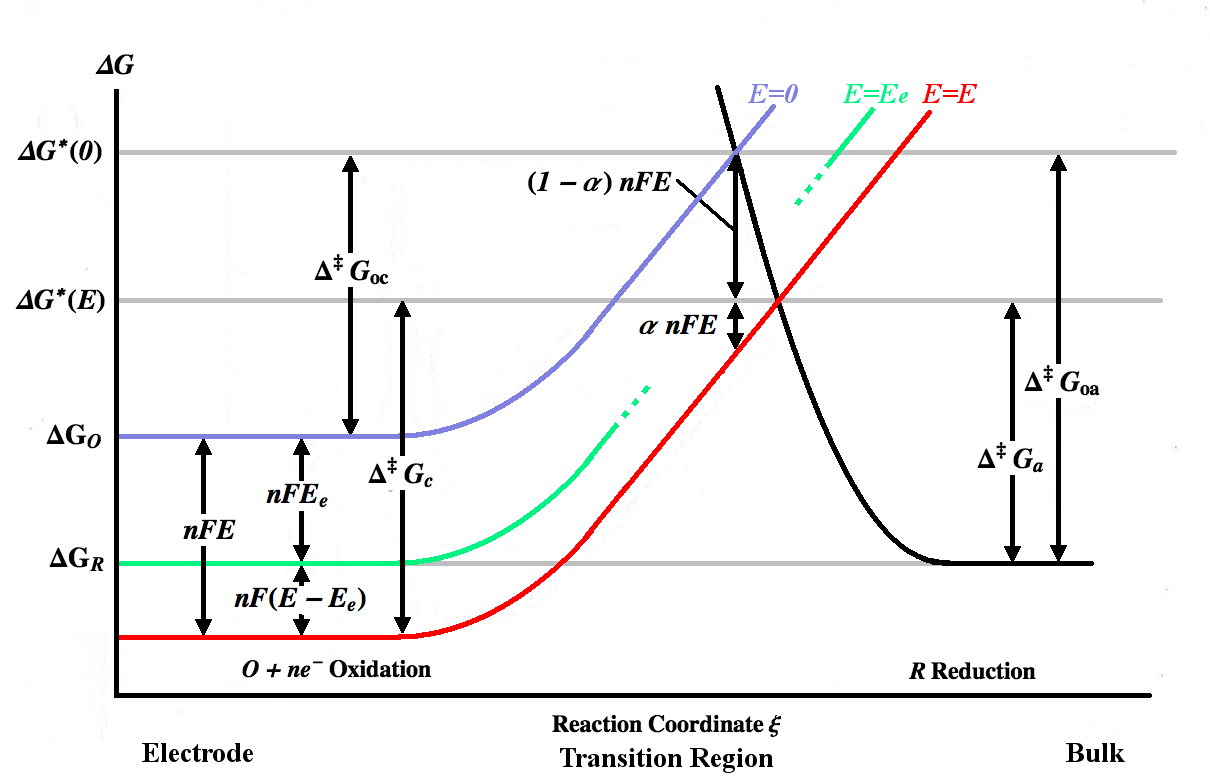
\includegraphics[width=13cm]{ButlerVolmerGibbsPlot.png}\\
    各物质的吉布斯自由能与反应坐标关系图。反应将朝着降低能量方向进行\\
    蓝色曲线为还原,红色曲线为氧化。绿色曲线说明了反应达到平衡。
    \caption{吉布斯自由能$\Delta G$与反应坐标$\xi$及电极电势$E$的关系\cite{Gibbs}}
    \label{fig:ButlerVolmerGibbsPlot}
\end{figure}

假设反应的速率常数由式~\ref{equation:Arrhenius}Arrhenius方程确定:
\begin{equation}
    \begin{aligned}
        k_ {f} = A_ {f} \ exp [-\Delta ^ {\ddagger} G_ {c} / RT]\\
        k_ {b} = A_ {b} \ exp [-\Delta ^ {\ddagger} G_ {a} / RT]%&是用于标注需要对齐的位置
    \end{aligned}
\end{equation}

其中$A_ {f}$与$A_ {b}$是与反应速度有关的常数。假设能量曲线在过渡区域中几乎是线性的,则可以用以下方式表示:
\begin{equation}
    \begin{aligned}
        &\Delta G = S_{c} \xi + K_{c} & \mbox{蓝色曲线}\\
        &\Delta G = S_{c} \xi + K_{c} -nEF \quad &\mbox{红色曲线}\\
        &\Delta G =- S_{a} \xi + K_{a} \quad &\mbox{黑色曲线}
    \end{aligned}
\end{equation}

这种简单情况下的电荷转移系数等效于对称系数,可以用能量曲线的斜率表示:
\begin{equation}
    \alpha=\frac{S_ {c}}{S_ {a} + S_ {c}}
\end{equation}

推导出:
\begin{equation}
    \begin{aligned}
        &\Delta ^{\ddagger }G_{c}=\Delta ^{\ddagger }G_{oc}+\alpha nFE\\
        &\Delta ^{\ddagger }G_{a}=\Delta ^{\ddagger }G_{oa}-(1-\alpha )nFE
    \end{aligned}
\end{equation}

为简洁起见,我们定义:
\begin{equation}
    \begin{aligned}
        &f_{\alpha }=\alpha nF/RT\\
        &f_{\beta }=(1-\alpha )nF/RT\\
        &f=f_{\alpha }+f_{\beta }=nF/RT
    \end{aligned}
\end{equation}

速率常数现在可以表示为:
\begin{equation}
    \begin{aligned}
        &k_{f}=k_{fo}e^{-f_{\alpha }E}\\
        &k_{b}=k_{bo}e^{f_{\beta }E}
    \end{aligned}
\end{equation}

其中零电位下的速率常数为:
\begin{equation}
    \begin{aligned}
        &k_{fo}=A_{f}e^{-\Delta ^{\ddagger }G_{oc}/RT}\\
        &k_{bo}=A_{b}e^{-\Delta ^{\ddagger }G_{oa}/RT}
    \end{aligned}
\end{equation}

现在我们可以将电流密度$j$写作外加电势$E$的函数\cite{CITEREFNewmanThomas-Alyea2004}:
\begin{equation}
    j=nF(c_{r}k_{bo}e^{f_{\beta }E}-c_{o}k_{fo}e^{-f_{\alpha }E})
\end{equation}

在一定的电压$E_{eq}$下,反应达到平衡,$vf$和$vb$相等
(如图~\ref{fig:ButlerVolmerGibbsPlot}绿色曲线表示)。
此时平衡电流是相等的,写成$j_o$,也就是交换电流密度。
我们定义过电位$\eta=E-E_ {eq}$,此时电流密度$j$可以表达为:
\begin{equation}
    j=j_{0}\cdot \left\{\exp \left[{\frac {\alpha _{a}zF\eta }{RT}}\right]-\exp \left[-{\frac {\alpha _{c}zF\eta }{RT}}\right]\right\}
    \label{equation:Butler_Volmer}
\end{equation}

这被称为Butler-Volmer方程,描述了在一个电极上的施加电势与电极电流的关系。